\chapter{Úvod}
Zpracování řeči hraje v dnešní době důležitou roli v mnoha rozličných oborech. Mezi jeden z hlavních úkolů bezesporu patří separace zdrojů v nějakém zaznamenaném signálu, který může být složen ze signálů N mluvčích, ale i nechtěného hluku okolí. Vyřešení problému je předpoklad k dalším úkonům jako identifikace konkrétního mluvčího nebo třeba přepis nějaké konverzace na text. Se stále se zrychlujícím vývojem počítačů a s jejich zvyšujícím se výkonem se do popředí dostávají metody zpracování řeči založené na neuronových sítích, které v mnoha ohledech předčily ostatní algoritmy strojového učení.

Separace mluvčích v časové doméně dosahuje mimořádných výsledků v porovnání s dosavadními metodami  založenými na převodu signálu z časové domény do frekvenční domény pomocí algoritmu STFT (Short--Time Fourier Transformation). Taková reprezentace signálu není optimální pro udržení časových závislostí, které jsou při zpracování řeči podstatné. V architektuře, která je navržena v referenční studii, je vstupní signál převeden do nezáporné reprezentace, která je optimální pro extrakci jednotlivých mluvčích. Silnou stránkou systému je hluboká architektura sítě, která lépe modeluje dlouhodobé závislosti v signálu. Zárověň se ale musí vypořádat s problémy, které hluboké neuronové sítě mohou přinášet.

Téma v oblasti strojového učení a neuronových sítí mě zaujalo, protože tento obor zažívá obrovský rozmach a pomalu se stává součástí téměř všech odvětví, a je tudíž velmi perspektivní pro další výzkum. Právě bakalářskou práci jsem vyhodnotil jako dobrou příležitost k tomu, se seznámit se s neuronovými sítěmi a možnost vyzkoušet si, jak se s nimi pracuje, jak se implementují modely za pomoci frameworku a jak náročná je aplikace na nějaký reálný problém.

\todo{spravit referenci na studii}
Mým úkolem v rámci práce je nastudovat si problematiku neuronových sítí a jejich základní principy, seznámit se problémem separace mluvčích pomocí neuronových sítí a následně implementovat síť podle architektury TasNet pro separaci mluvčích v časové doméně, která byla navržena a popsána ve studii \ref{referencni_studie}. Potom tuto neuronovou síť natrénovat s různými kombinacemi hodnot hyperparametrů, které ovlivňují velikost sítě  její vlastnosti, a nakonec porovnat přesnost a kvalitu separace mezi jednotlivými, různě velkými sitěmi a mezi výsledky studie. Přesnost separace je vypočítána pomocí míry si--snr, udávající poměr mezi chtěným signálem a hlukem na pozadí. Sítě budou testovány a vyhodnocovány na testovací množině jednokanálových směsí dvou mluvčích.

V první části práce, kterou pokrývá kapitola \ref{neuronovky}, jsou popsány základní prvky neuronových sítí, struktura umělého neuronu, jeho vstupy a výstupy, váhy a role aktivační funkce. V návaznosti na to jsou popsány neuronové sítě feedforward, které se skládají z vrstev neuronů. Dále je vysvětlen proces učení, který se skládá z několika kroků -- výpočet výstupu sítě, výpočet chyby a úprava vah, kde hraje podstatnou roli metoda backpropagation. Nakonec je zmíněn typ sítí feedforward -- konvoluční neuronové sítě, které fungují na základě konvoluční operace. Konvoluční sítě se používají nejčastěji pro zpracování obrazu kvůli vlastnostem, které umožňují extrahovat příznaky s různou úrovní složitosti od základních útvarů jako úsečka, barva a podobně až po komplexnější příznaky - třeba celý obličej. Tohoto lze využít i při zpracování zvuku, kde jsou tyto extrahované příznaky jednorozměrné.

Druhá část, kapitola \ref{tasnet}, je věnována architektuře TasNet. Prvně je zmíněn konvoluční auto--enkodér a jeho princip. Dál je popsána podoba separačního modulu, jeho princip a konvoluční bloky, ze kterých je poskládán. Tento blok obsahuje konvoluční vrstvy, normalizace a aktivační funkce. Bloky jsou skládány za sebe se zvyšující se časovou dilatací, čemuž se říká TCN (Temporal Convolutional Network). 

Kapitola \ref{implementace} se zabývá implementací neuronové sítě a jejím trénováním. Je popsána a zdůvodněna volba frameworku, implementace sítě a struktura zdrojového kódu. Pro usnadnění často se upakujících úkonů jsem vytvořil pár pomocných scriptů, které jsou zde také popsány. 
Model prošel během implementace několika úpravami. Pro účely trénování a validace byly vstupní nahrávky rozdělovány na čtyřsekundové segmenty. Pro testování byly používány nahrávky celé. V této kapitole je popsán průběh trénování sítí, výsledky a použité nástroje.

V poslední části, která je pokryta v kapitole \ref{experimenty} jsou shrnuty experimenty s modelem a vyhodnocení výsledků, v rámci něhož je zkoumán vliv hyper-parametrů na učení sítě, na výsledky a přesnost separace v závislosti na zvolených parametrech nebo počtu konvolučních bloků. Výstup sítě v podobě separovaných mluvčích je porovnán také s výsledky referenční studie. Kvalita separace, neboli přesnost, je vypočítána pomocí si--snr metriky která udává poměr zastoupení chtěného signálu a hluku na pozadí. Je zde vyhodnoceno, jaký vliv má velikost sítě na přesnost separace a jsou zde shrnuty jednotlivé výsledky.

%----------------------------------------------------------------------------------------------------------------------------------------------------------------------
\chapter{Neuronové sítě}
\label{neuronovky}
V dnešní době zažívají neuronové sítě díky výkonosti počítačů velký rozmach. Jejich využití prostupuje skrze mnohé vědní obory a dokáží řešit celou řadu problémů, ve kterých dosahují výborných výsledků, které zdaleka předčily dosavadní postupy. 

Neuronové sítě (\textit{artificial neural networks}) jsou výpočetní model, který je inspirovaný strukturou lidského mozku, ve kterém je obrovské množství propojených a komunikujících neuronů. Ty se skládají ze vstupních dendridů, výstupních axonů a samotného těla neuronu. Na základě vnitřního potenciálu a vstupních hodnot je po přesažení prahové hodnoty neuron vybuzen a je vyslán signál na výstupní axon. Signál je nakonec předán dalším neuronům skrze jejich vstupní dendridy\cite[p.~65--66]{mitdeeplearning_small}.

Účelem neuronové sítě je naučit se plnit zadanou úlohu. Rozdíl oproti běžným algoritmům je ale ten, že způsob, jakým síť má problém řešit, není explicitně naprogramován, ale je postupně naučen. Základní způsoby učení jsou s učitelem (\textit{supervised}) a bez učitele (\textit{unsupervised}). 

\textbf{Učení s učitelem} spočívá v \todo{bla bla (dve tri vety)}.
\textbf{Učení bez učitele} spočívá v \todo{bla bla (dve tri vety)}.

Mezi problémy, které se dají řešit neuronovými sítěmi patří klasifikační a regresní problémy. Konkrétní příklad z oblasti klasifikace může být rozpoznávání objektů na obraze, psaného písma nebo detekce obličejů na videu, ale i mnohé aplikace ve zpracování řeči. 




\section{Organizace feedforward sítí}
Feed forward neuronové sítě jsou typ umělých neuronových sítí, kde se nevyskytují cykly ve výpočetním grafu, tedy zpětná propojení vrstev, takže informace se pohybuje pouze jedním směrem, od vstupní vrstvy přes skryté vrstvy až do vrstvu výstupní. Sítě, které obsahují cykly, se nazývají rekurentní. Rozdíl znázorňuje obrázek \ref{fig:netcomparison}.

\begin{figure}[H]
    \centering
    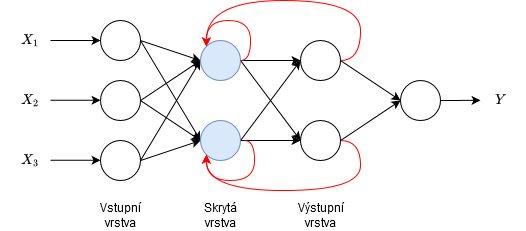
\includegraphics[scale=0.5]{obrazky-figures/feedforward_vs_recurrent.png}
    \caption{\label{fig:netcomparison}Příklad grafu feed forward sítě a rekurentní neuronové sítě. Lze si všimnout orientace šipek u feed forward sítě, které směřují pouze jedním směrem, zatímco u rekurentní sítě šipky směřují i k předešlým uzlům grafu.}
\end{figure}

Struktura neuronové sítě je organizována do vrstev, které se skládají z neuronů. Feedforward síť je tvořena třemi typy vrstev (viz obrázek \ref{fig:mlp}). Každá vrstva může obsahovat až $n, n \in \mathbb{N}\setminus\{0\}$ neuronů. Vstupní vrstva slouží k předání hodnot do sítě, ale nijak tyto hodnoty nemodifikuje. Nezměněné jsou zkopírovány do první skryté vrstvy. Následují skryté vrstvy, z nichž poslední je napojena na výstupní vrstvu. Ta má obvykle méně neuronů než předešlé vrstvy a hodnoty na výstupu mohou představovat třídy, do kterých má být klasifikován vstup. S počtem jednotlivých vrstev souvisí pojem hloubka sítě, která je rovna počtu všech vrstev neuronové sítě od vstupní až po výstupní vrstvu. Pojmem hluboká neuronová síť se označuje taková síť, která má dvě nebo více skrytých vrstev. Vrstvy se ještě dále rozdělují na plně propojené, pooling, s přeskočením či na konvoluční vrstvy.

\begin{figure}[H]
    \centering
    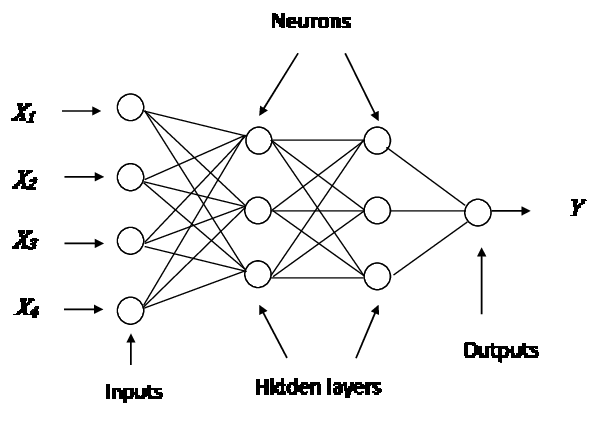
\includegraphics[scale=1.3]{obrazky-figures/mlp.png}
    \caption{\label{fig:mlp}Schéma neuronové sítě, která má 2 skryté vrstvy}
\end{figure}



\section{Umělý neuron}
Základní stavební jednotka neuronových sítí je umělý neuron (\textit{artificial neuron}) (viz obrázek \ref{fig:neuron}). Tento model je založen na principu reálných neuronů, které se nacházejí v organizmech. Umělý neuron obsahuje libovolně mnoho vstupních propojení, přes které se mu předávají data v podobě vstupního vektoru $\overrightarrow{x} = [x_1, x_2, \dots, x_n], x_n \in \mathbb{R}$. Sám neuron obsahuje hodnotu bias $b \in \mathbb{R}$ a vektor vah $\overrightarrow{w} = [w_1, w_2, \dots, w_n], w_n \in \mathbb{R}$, jenž je upravován během trénování neuronu.

Výstupní hodnota závisí na vstupních datech, aktuálním vnitřním stavu (hodnoty vah a biase) a na zvolené aktivační funkci. Vstupní hodnoty jsou váhovány, což znamená, že každá vstupní hodnota je vynásobena s váhou na daném vstupním spojení. S použitím definovaných vektorů lze napsat, že vstupní vektor je vynásoben s vektorem vah.

\begin{figure}[H]
    \centering
    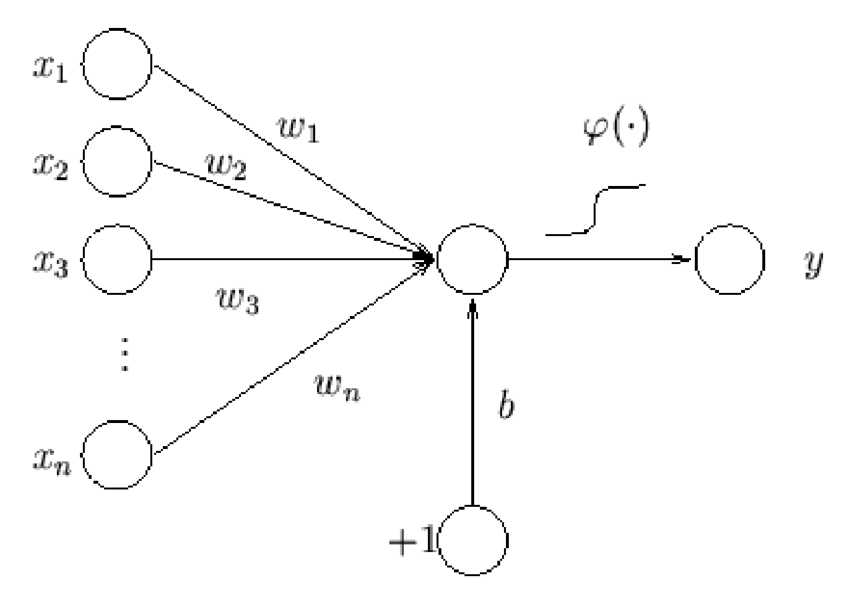
\includegraphics[scale=0.35]{obrazky-figures/perceptron.png}
    \caption{\label{fig:neuron}Schéma umělého neuronu}
\end{figure}

Hodnota bias $b$, která je přičtena k sumě násobků vah a vstupních hodnot, je prahová hodnota modifikující dobu, kdy se aktivuje neuron a změní svůj výstup. Matematicky to znamená, že s grafem aktivační funkce horizontálně pohybuje doleva nebo doprava v závislosti na tom, je-li hodnota biasu pozitivní nebo negativní. Toto posunutí je znázorněno na obrázku \ref{fig:bias}. V závislosti na řešeném problému může být žádoucí, aby i hodnota bias byla modifikována během učení společně s ostatními váhami. V opačném případě je hodnota nastavena pevně na nějakou konstantní hodnotu, obvykle na hodnotu jedna.

\begin{figure}[H]
    \centering
    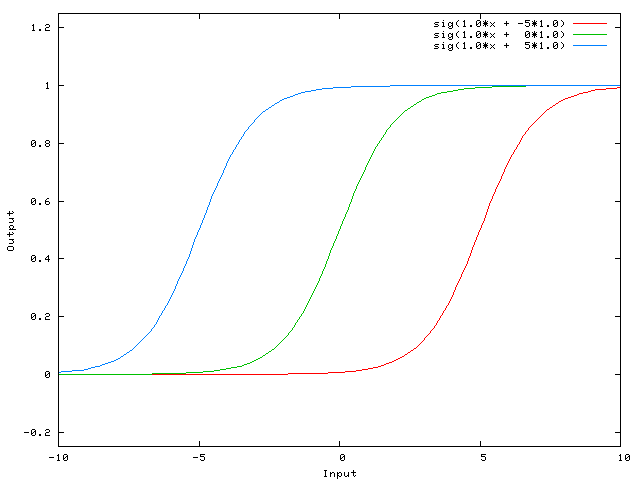
\includegraphics[scale=0.4]{obrazky-figures/bias.png}
    \caption{\label{fig:bias}Vliv hodnoty bias na aktivační funkci}
\end{figure}




Výstup neuronu se vypočítá jako
\begin{equation}
	y = f\big((\sum_{k=1}^n w_kx_k) + b\big)
\end{equation}
kde $f$ je nějaká aktivační funkce, $x_k \in \mathbb{R}$ je vstupní hodnota, $w_k \in \mathbb{R}$ je váha, kterou se vstupní hodnota vynásobí a $b \in \mathbb{R}$ je hodnota bias, která je přičtena k celkové sumě předtím, než je výsledek předán aktivační funkci.





\section{Aktivační funkce}
Aktivační, neboli prahová funkce určuje výstupní hodnotu neuronu. Funkce se vybírá na základě problému, který se má neuronová síť naučit řešit. Správná volba prahové funkce vede k lepší konvergenci učení sítě. Naopak špatná volba může vést ke stále větší odchylce od správného řešení -- může divergovat. Povaha problému může vyžadovat specifické vlastnosti aktivační funkce - lineární nebo nelineární. Pro nestandardní problémy je obvykle potřeba experimentálně zjistit, která funkce bude nejlépe vyhovovat danému problému. 

Pokud by veškeré aktivační funkce v modelu byly lineární, tak celkové mapování sítě by bylo omezeno pouze na lineární mapování vstupu na výstup. Reálné problémy ale lineární obvykle nejsou a v případě pokusu modelovat takovým modelem nelineární vztahy by vedlo k velice nepřesným výsledkům, který by byl zapříčiněn podučením (\textit{underfitting}), což znamená, že model, který se učí zakódovat nějaký vzor v datasetu, je příliš jednoduchý. Proto je potřeba zavést do modelu i nelineární aktivační funkce, které tento problém řeší\cite[p.~77--78]{mitdeeplearning_small}.

Z pohledu učení je také důležité, aby aktivační funkce byla diferencovatelná. To umožňuje použití učících metod založených na výpočtu gradientu.



\subsection*{Sigmoid}
\begin{equation}
  f(x) = \frac{1}{1+\exp(-z)}
\end{equation}

\todo{popsat}

\begin{figure}[H]
    \centering
    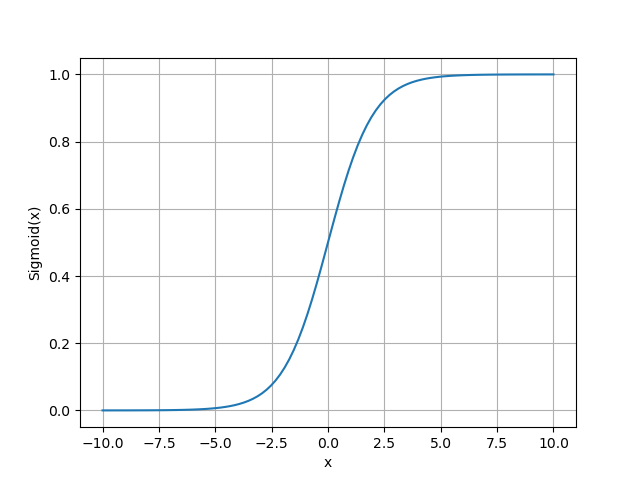
\includegraphics[scale=0.18]{obrazky-figures/sigmoid.png}
    \caption{\label{fig:sigmoid}Graf aktivační funkce sigmoid}
\end{figure}



\subsection*{Softmax}
\begin{equation}
  f(x) = \frac{1}{1+\exp(-z)}
\end{equation}

\todo{popsat}

\begin{figure}[H]
    \centering
    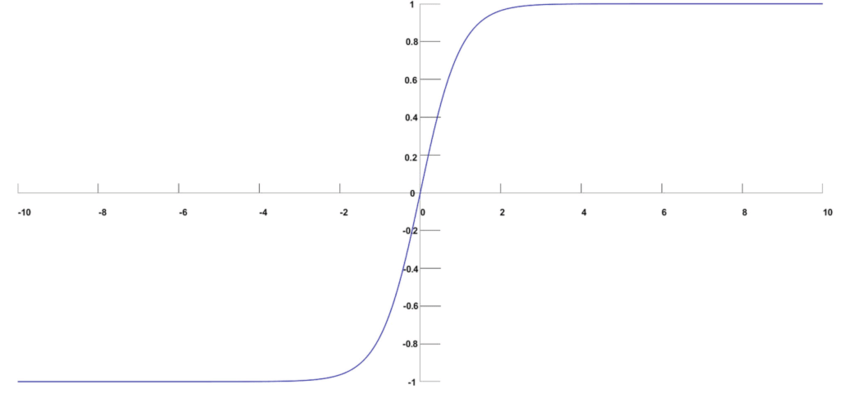
\includegraphics[scale=0.35]{obrazky-figures/softmax.png}
    \caption{\label{fig:softmax}Graf aktivační funkce softmax}
\end{figure}




\subsection*{ReLU}
Rectified Linear Unit je nejčastěji používaná aktivační funkce. Vyžaduje-li neuronová síť nějakou nelinearitu, je ReLU pro většinu případů ideální. Pro každou zápornou hodnotu $x$ vrací $0$ a pro kladnou hodnotu $x$ vrací tutéž hodnotu $x$, jak udává rovnice 
\begin{equation}
   f(x)=max(0,x)
\end{equation}

\begin{figure}[H]
    \centering
    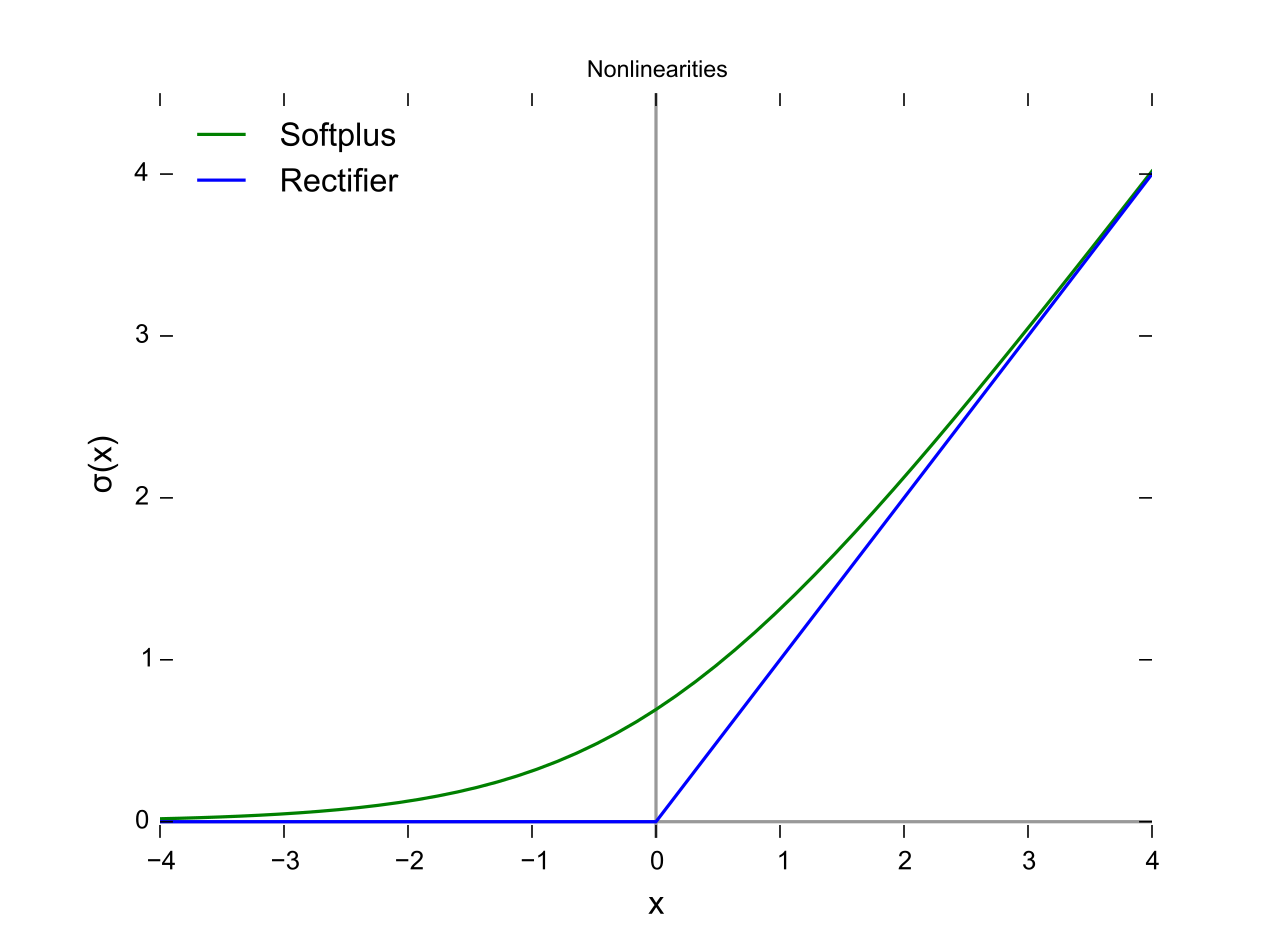
\includegraphics[scale=0.2]{obrazky-figures/ReLU.png}
    \caption{\label{fig:relu}Graf aktivační funkce ReLU}
\end{figure}




\subsection*{PReLU}
Parametrizovaná ReLU je nelineární aktivační funkce, která se používá v případě, že chceme produkovat na výstup malý nenulový gradient i v případě záporné vstupní hodnoty $x$. V tom případě je vstupní hodnota vynásobena parametrem $\alpha$ a to představuje výsledek. Parametr $\alpha$ se společně s ostatními váhami učí během učícího procesu.
\begin{equation}
  f(x) =
  \begin{cases}
    x & \text{if } x \geq 0 \\
    {\alpha}x & \text{if } x < 0
  \end{cases}
\end{equation}

\begin{figure}[H]
    \centering
    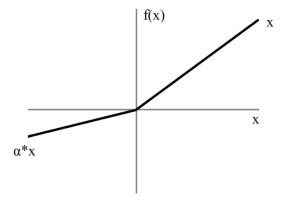
\includegraphics[scale=1.4]{obrazky-figures/prelu.jpg}
    \caption{\label{fig:prelu}Graf aktivační funkce PReLU}
\end{figure}



Síť složená z jediného neuronu by byla omezena pouze na klasifikaci lineárně separovatelných dat. To jsou taková data, která lze rozdělit, existuje-li alespoň jedna přímka v rovině taková, že na jedné straně přímky jsou všechna data klasifikována do první třídy, a na druhé straně data klasifikována do třídy druhé, jak lze vidět na obrázku \ref{fig:linear_separable}.

\begin{figure}[H]
    \centering
    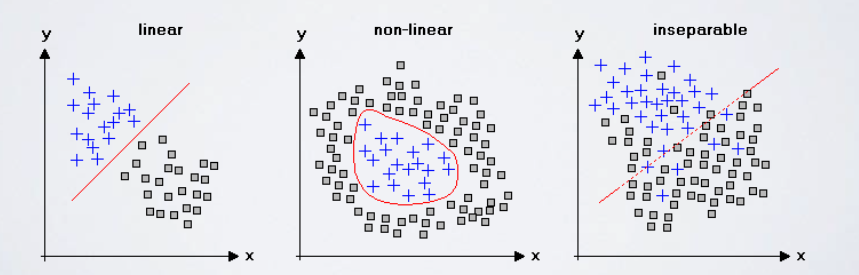
\includegraphics[scale=0.38]{obrazky-figures/linear_separable.png}
    \caption{\label{fig:linear_separable}Lineárně separovatelná (vlevo) a neseparovatelná (vpravo) data} 
\end{figure}

Mějme množinu dat, kterou tvoří dvě rozdílné třídy objektů $\Omega_1, \Omega_2 \subset \mathbb{R}^m$. Třídy jsou lineárně separovatelné, jestliže existuje $w \in 
\mathbb{R}^m$ a $\theta \in \mathbb{R}$ takové, že 
\begin{equation}
   \forall x \in \Omega_1 : x^Tw > \theta
\end{equation}
\begin{equation}
   \forall x \in \Omega_2 : x^Tw < \theta
\end{equation}

Problém lze zobecnit tak, že řešením bude separace tříd pomocí hyper roviny v prostoru $\mathbb{R}^m$, jak zachycuje obrázek \ref{fig:hyperplane_separable}
\cite{linearseparability}.

\begin{figure}[H]
    \centering
    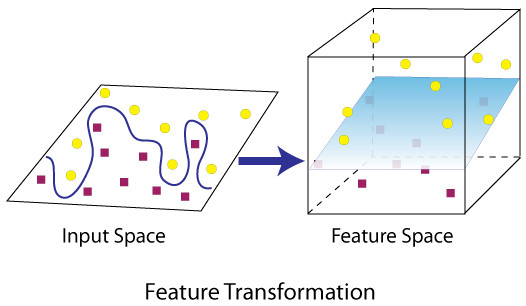
\includegraphics[scale=0.8]{obrazky-figures/hyperplane_separable.jpeg}
    \caption{\label{fig:hyperplane_separable}Separace pomocí hyper roviny} 
\end{figure}

Neuron se nedokáže ale naučit klasifikovat třeba funkci XOR, protože ta není lineárně separovatelná. Byly by zapotřebí minimálně dvě přímky pro rozdělení dat, jak zobrazuje obrázek \ref{fig:xor}\todo{ocitovat xor}.  

\begin{figure}[H]
    \centering
    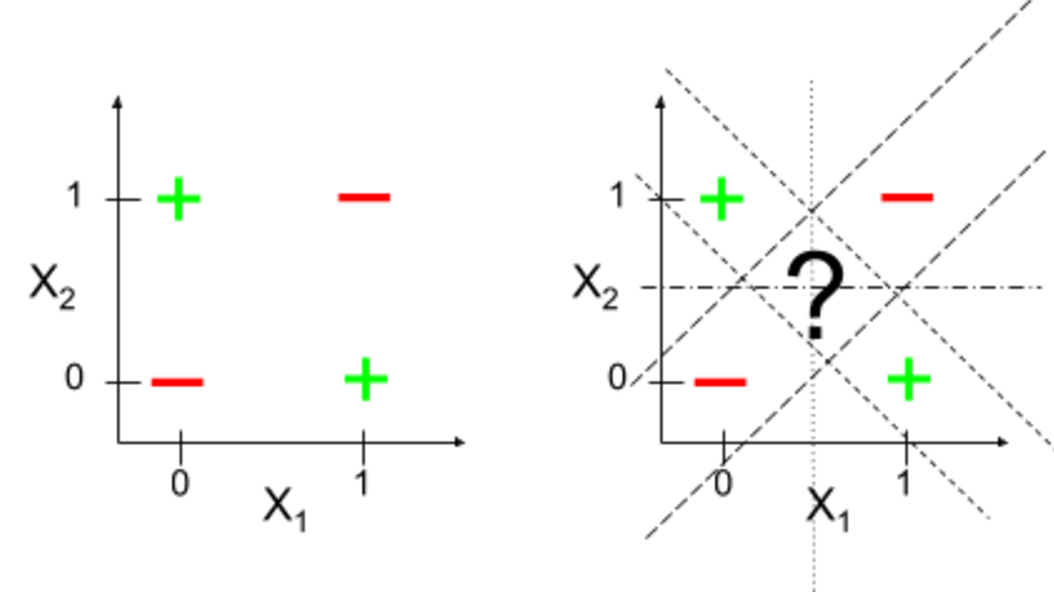
\includegraphics[scale=0.3]{obrazky-figures/xor.png}
    \caption{\label{fig:xor}Graf funkce XOR, jejíž výstup není lineárně separovatelný} 
\end{figure}

K překonání tohoto problému se neurony spojují do podoby neuronové sítě, která dokáže řešit libovolně komplexní problémy.




\section{Hyperparametry}
\todo{co to je, ze se to nastavuje pred trenovanim site, neni to meneno behem trenovani... learning rate, X, R, stride, padding, receptive field, ...}




\section{Učení neuronových sítí}
\todo{nepřejmenovat to na cz?}
\todo{v ramci tohoto proces uceni, cil uceni a objektivni funkce, MLP, }

Feedforward sítě (MLP) jsou nejzákladnější modely hlubokého učení. Cílem takové neuronové sítě je aproximovat nějakou funkci $f^\ast$. Síti je předána vstupní hodnota $x$, pro kterou síť definuje mapování na výstupní hodnotu jako $y = f(x; \theta)$, kde $\theta$ je parametr, který se síť učí tak, aby dosáhla nejlepší aproximace funkce. \cite[p.~163]{mitdeeplearning}.


\subsection{Objektivní funkce}
= cost funkce
-popis, co to je, k cemu to je, proc to je...

\subsection*{MSELoss}
- vzorecek
\subsection*{Cross Entrophy}
- vzorecek


\subsection{Optimalizační algoritmy}
 [1 deep learning str 301]
 Mozna kaslat...

\subsection*{Adam}
Adam je jeden z algoritmů s adaptivním učením. Jeho název byl odvozen z fráze "adaptive moments".  [1 deep learning str 301]
Mozna kaslat.


\subsection{Backpropagation}
- zpetne sireni chyby
- adaptacni algoritmus, podil neuronu na chybe,
- 3 opakujici se faze uceni:

\todo{dodelat zde podkapitoly v lepsim poradi}

1) feedforward - dopredu
2) zpetne sireni chyby - Backpropagation
3) uprava vah a biasu na zaklade chyby pomoci gradient descent
- chain rule



\subsection*{Gradient descent}

\subsection{Overfitting a generalizace}


\section{Konvoluce a konvoluční neuronové sítě}
Konvoluční neuronové sítě jsou typ feedforward sítí.
\begin{figure}[H]
    \centering
    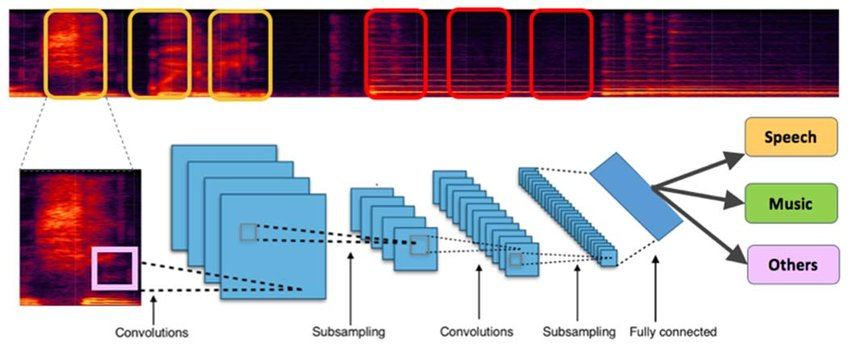
\includegraphics[scale=0.5]{obrazky-figures/conv_nn_audio.jpg}
    \caption{\label{fig:conv_nn}Konvoluční neuronové sítě}
\end{figure}


\subsection{Konvoluce}
Diskrétní konvoluce je definována jako

%\begin{equation}
%   (f \star g)_k = \sum_{i=-\inf}^\inf f_i * g_{k-i} = \sum_{i=-\inf}^\inf f_{k-i} * g_{i}
%\end{equation}

kde $\star$ je konvoluční operátor, $f$ je funkce signálu, funkce $g$ je konvoluční jádro a $f_i$ a $g_i$ jsou hodnoty funkce na indexu $i$.






%----------------------------------------------------------------------------------------------------------------------------------------------------------------------
\chapter{TasNet - Time--Domain Audio Separation Network}
\label{tasnet}
\todo{Architektura full -- obrázek, bloky...}
\begin{figure}[H]
    \centering
    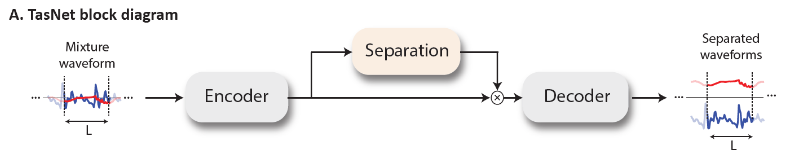
\includegraphics[scale=0.5]{obrazky-figures/tasnet-pipe.png}
    \caption{\label{fig:tasnet-pipe}Zjednodušený model architektury}
\end{figure}


\section{Konvoluční auto--enkodér}
\todo{Konvoluční autoenkodér, vstup, výstup...}

- schema bez separacniho modulu
- non negative representation of audio
\begin{figure}[H]
    \centering
    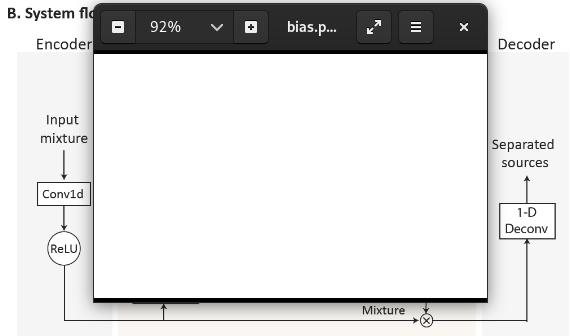
\includegraphics[scale=0.5]{obrazky-figures/tasnet-autoencoder.png}
    \caption{\label{fig:tasnet-autoencoder}Schéma konvolučního autoenkodéru}
\end{figure}


\section{Separační modul}
- odhad masek pro jednotlive mluvci
- schema se separacnim modulem
\begin{figure}[H]
    \centering
    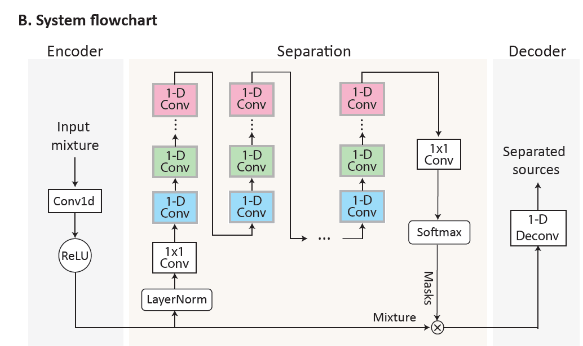
\includegraphics[scale=0.6]{obrazky-figures/tasnet-architecture.png}
    \caption{\label{fig:tasnet-modul}Schéma architektury TasNet}
\end{figure}


\subsection{Konvoluční bloky}
- Z čeho se skládá -- konvoluční vrstvy, normalizace
- diagram konv bloku.
- Mozna: Dilatace a time perception
\begin{figure}[H]
    \centering
    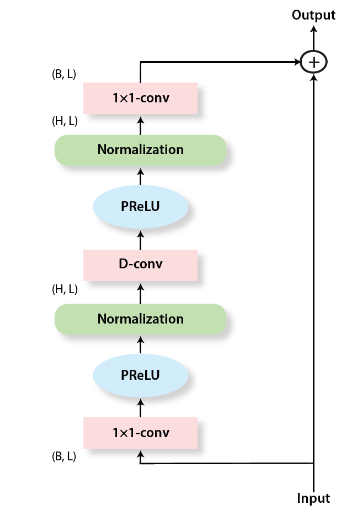
\includegraphics[scale=0.5]{obrazky-figures/conv-res-block.png}
    \caption{\label{fig:tasnet-convblock}Jeden konvoluční blok}
\end{figure}


%----------------------------------------------------------------------------------------------------------------------------------------------------------------------



\chapter{Implementace a trénování sítě}
\label{implementace}
Pozn: colab, pytorch, stroj, bash, hyperparams, vykon a cas trenovani, seg--len, popis trid.

\section{Implementace modelu}
- pytorch, scripty, python3, bash, tridy, moduly, parametry a volby spusteni.

\section{Dataset}
\todo{Ukazat zde vykreslenou vlnu nahravek mix, s1, s2}
\todo{popsat co je dataset a k cemu to slouzi}
Trénování a vyhodnocení modelu proběhlo na množině jednokanálových nahrávek směsí dvou mluvčích. Množina byla vygenerována náhodným výběrem různých mluvčích z Wall Street Journal (WSJ0) a vytvořením směsi. Celková délka trénovacích dat je přes 10 hodin a přes 6 hodin validačních dat. Nahrávky jsou převzorkovány na 8kHz a během trénování zarovnány na zero means a jednotkovou varianci[studie str 5 Dataset][49 - ze studie odkaz na script na generovani a popis na netu].
\begin{figure}[H]
    \centering
    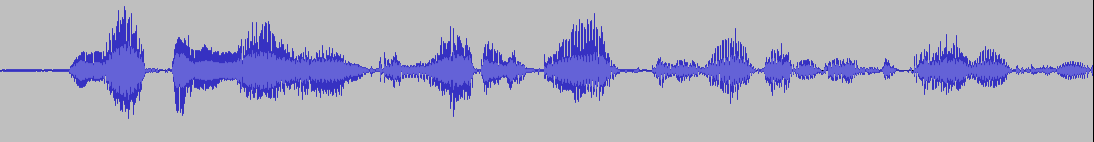
\includegraphics[scale=0.35]{obrazky-figures/dataset-mix.png}
    \caption{\label{fig:ref-mixture}Ukázka nahrávky směsi dvou mluvčích}
\end{figure}
\begin{figure}[H]
    \centering
    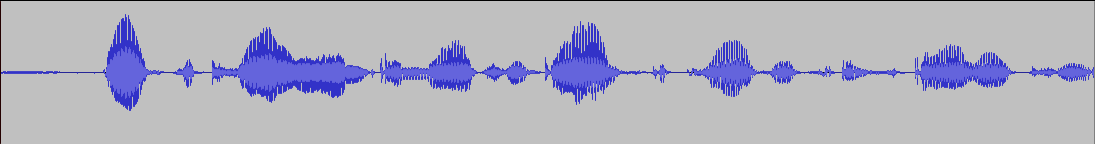
\includegraphics[scale=0.35]{obrazky-figures/dataset-s1.png}
    \caption{\label{fig:ref-s1}První mluvčí ze směsi}
\end{figure}
\begin{figure}[H]
    \centering
    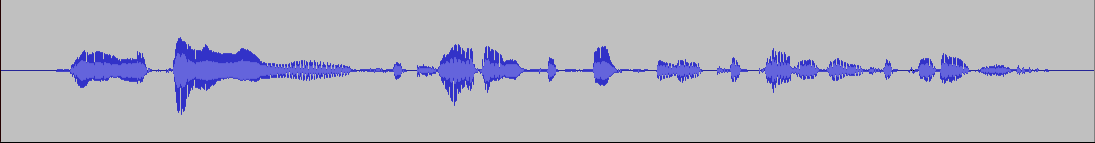
\includegraphics[scale=0.35]{obrazky-figures/dataset-s2.png}
    \caption{\label{fig:ref-s2}Druhý mluvčí ze směsi}
\end{figure}
Lze si všimnout, že sečtením signálů separovaných mluvčích na obrázku \ref{fig:ref-s1} a \ref{fig:ref-s2} dostaneme přesně signál směsi, což lze vyjádřit vztahem
\begin{equation}
  x[t] = \sum_{i=1}^C s_i[t]
\end{equation}
, kde $x[t] \in \mathbb{R}^{1 \times T}$ je diskrétní signál směsi a $s_i[t] \in \mathbb{R}^{1 \times T}$, kde $i = 1,\ldots,C$, je jeden z $C$ zdrojů[cite studie str3 vlevo]. 
\todo{doplnit info o zero means a jendotkove varianci}

\section{Trénování}
\begin{figure}[H]
    \centering
    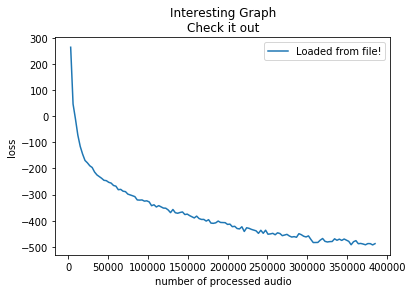
\includegraphics[scale=0.55]{obrazky-figures/some-loss.png}
    \caption{\label{fig:somelossTODO}Příklad grafu loss hodnoty během učení}
\end{figure}

\begin{figure}[H]
    \centering
    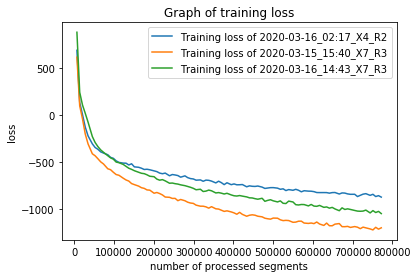
\includegraphics[scale=0.55]{obrazky-figures/loss_triple.png}
    \caption{\label{fig:somelossTODO2}Hodnota loss při trénování modelů s různou velikostí hyperparametrůx}
\end{figure}

\subsection{Význam validační množiny v trénování}
Většina algoritmů strojového učení má nějakou sadu hyperparametrů, kterou je upravováno chování algoritmu. Hodnoty hyperparametrů obvykle bývají nastavovány ručně ještě před spuštěním procesu učení a hodnota se v průběhu nemění, protože hodnoty by bylo obtížné optimalizovat. 
Některá nastavení se nicméně mohou stát hyperparametrem a být upravována během trénování, ale není vhodné je měnit na základě výsledku učení na trénovací sadě, protože by mohlo dojít k přetrénováníoverfitting) v důsledku \todo{CEHO??}. Pro tento případ potřebujeme validační sadu, která je odlišná od trénovací sady.
Po každém zpracování trénovací sady následuje validační sada, po jejímž skončení jsou optimalizovány hyperparametry[][].

\todo{[kniha 117-118] kap 5.3 = Hyperparameters and validation set} 
\todo{najit jeste nejakej zdroj s popisem a pripadne nejaky zajimavejsi info.}

\section{Vyhodnocovací metriky}
- minimalizovat objektivni-hodnotici funkci sisnr.
\subsection{Signal to noise ration}
\subsection*{Source Distortion Ratio -- SDR}
\subsection*{Artifacts Ratio -- SAR}
\subsection*{Inference Ratio -- SIR}



%----------------------------------------------------------------------------------------------------------------------------------------------------------------------


\chapter{Experimenty a vyhodnocení}
\label{experimenty}
- trenovani s ruznymi hyperparametry, uspesnost a tabulky s hyper parametry a dosazenymi vysledky a hodnotami sisnr, sdr atd.
- model size comparison.
- porovnani s vysledky ze studie
- obrazky separovanych mluvcich - signalu.
- spektra
- grafy trenovani loss a vysledkuu.
- pametova narocnost modelu


\section{Možná rozšíření a navrhnutá vylepšení}
- variabilnější dataset, mikrofony, šum a bordel prostředí
- separace více mluvčích
- hlučné prostředí
- identifikace konkrétního řečníka
- realtime separace

%----------------------------------------------------------------------------------------------------------------------------------------------------------------------

\chapter{Závěr}
\label{zaver}
- co jak dopadlo, vysledky a vyhodnoceni velikosti modelu a jaky byl nejlepsi,...

Cílem práce bylo implementovat síť podle architektury TasNet pro separaci mluvčích v časové doméně a porovnat vliv velikosti sítě na kvalitu separace. Síť byla implementována za pomoci frameworku pytorch a jazyku python a natrénována na datasetu obsahujícím jednokanálové směsi dvou mluvčích. Trénování proběhlo na \todo{X} modelech, které se od sebe lišily počtem opakujících se konvolučních bloků, velikostí časové dilatace a délkou vstupních segmentů směsí. Pro účel vyhodnocení modelů byla použita metrika si-snr, která udává poměr chtěného signálu ku šumu na pozadí, tedy obecně kvalitu separace. 

Experimenty ukázaly, že během testování nejlépe dopadla síť, která měla 8 konvolučních bloků po 4 opakováních, s délkou vstupního segmentu $L=2$ sekundy. Tento model dosáhl po 100 epochách trénování hodnoty až \todo{13,4} a tím se stal nejúspěšnějším modelem. Při fyzickém poslechu separovaných nahrávek bychom neslyšeli téměř žádný náznak druhého mluvčího. Oproti tomu, nejméně přesný model měl pouze 4 konvoluční bloky, 2 opakování a při délce segmentů $L=4$ sekundy dosahoval hodnoty SDR pouze \todo{9.2}.

Zkoušel jsem separovat také nahrávky, které byly úplně mimo dataset, ale výsledek se nedá hodnotit jako úspěšný, jelikož hraje velkou roli prostředí, mikrofon, šum v pozadí a další vlivy, na které byla neuronová síť naučena. Tento problém by se dal překonat rozšířením trénovacího datasetu o větší škálu nahrávek mluvčích, které by byly pořízeny z různých zařízení v různě rušném prostředí.

\todo{Doplnit ještě neco eh}

Mozna.


